\documentclass[technical_document.tex]{subfiles}
\begin{document}

Eva�s electrical system consists of three subsystems. First there is the power electronics part built around the battery and the DC power input. This provides the necessary power to the other subsystems: the motor electronics and the mainboard. 

\section{Power Electronics}

Eva can be powered either from a $12V$ battery or a $12V DC$ power input. She has a control panel behind the front bumper from where you can switch between battery power and net power. 
There is room for one big $17AH$ lead acid battery between Eva�s wheels as well as a smaller $7AH$ battery on the laptop level. The batteries cannot be active simultaneously. There is a switch to select the battery, which has to be used.  The main switch can shut down both battery and wall power at once.
 
 \begin{figure}[ht!]
	\centering
	\mbox{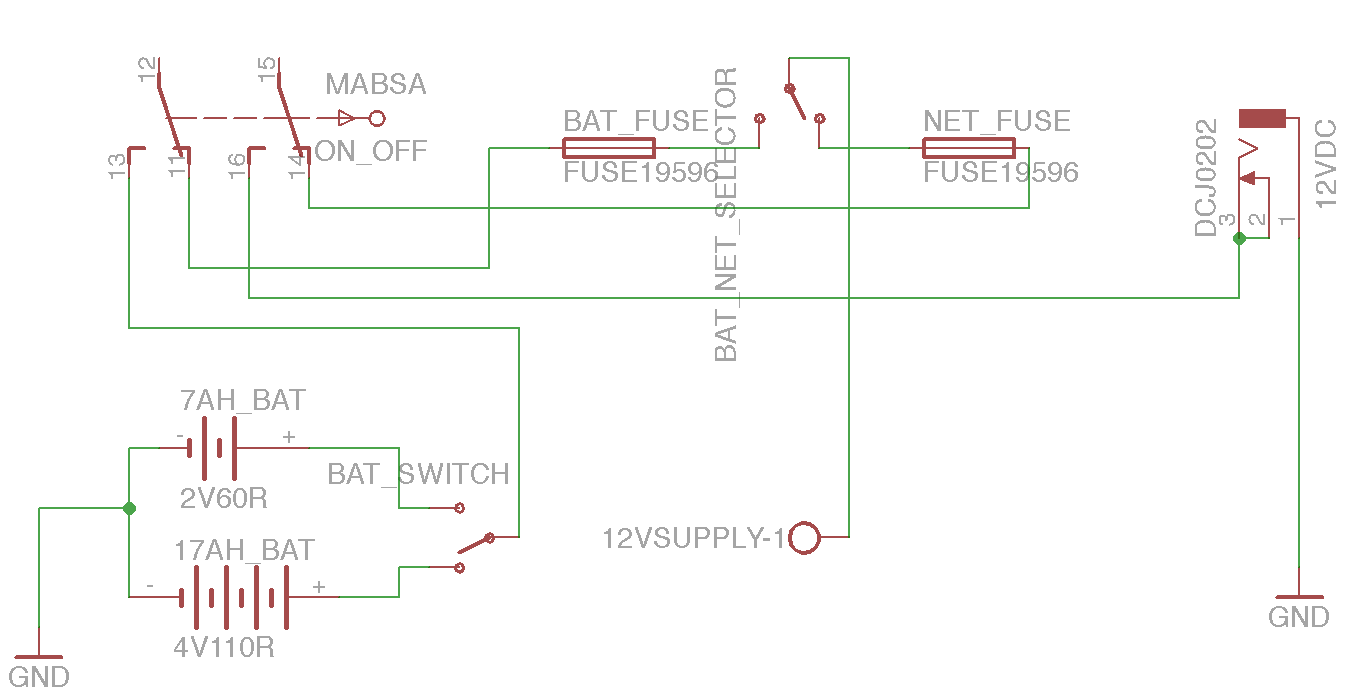
\includegraphics[scale=1.0]{Images/power_system.png}}
	\caption{Power system schematic}
	\label{fig:power_system}
\end{figure}
 
\section{Motor Electronics}

\subsection{Configuration}
Eva sports a total of seven motors and three servos. Two Dynamixels actuate the head. The mobile base, the arm and the gripper have motors controlled by three 3mxl boards. The 3mxl boards are daisy chained on the RS485 bus and accessible via one USB port. A separate USB port connects the Dynamixels� RS485 bus. 
We encountered problems talking to the 3mxl and Dynamixel over one bus. So we separated them. However it should be possible to use them all on one bus while using Shared Serial in ROS.
Table \ref{tab:motorConfiguration} shows an overview of the motors and the ID�s they listen to. The baud rate for the 3mxl serial connections is $921.6 kBaud$. The Dynamixels connect at $1.0 MBaud$.

\begin{table}[h]
\centering
  \begin{tabular}{| l | c | c | c | r |}
    \hline
    {\bf Motor} & {\bf ID} & {\bf Type} & {\bf Emergency stop} & {\bf Angle limits}	\\ \hline
    Head pan motor 	& 	104 & 	Dynamixel & -	& Software limits	\\ \hline
    Head tilt motor 	&	105 &	Dynamixel & -	& Software limits		\\ \hline
    Left Wheel motor   &	106 & 	3mxl &		power and 3mxl	& -	\\ \hline
    Right wheel motor &	107 & 	3mxl &		power and 3mxl	& -	\\ \hline
    Gripper motor	 & 	109 &	3mxl &		-	& -	\\ \hline
    Shoulder motor 	 &	110 &	3mxl &		power and 3mxl	& Software and hardware limits \\ \hline
    Elbow motor 		 &	111 &	3mxl &		3mxl	& Software and hardware limits	\\ 
    \hline
  \end{tabular}
\caption{Motor configuration}
\label{tab:motorConfiguration}
\end{table}



\newpage
\subsection{Safety measures}
The emergency stop affects the wheel and arm motors. When the emergency button is pushed the relays will cut the power to the motors and the 3mxl is signaled to stop driving the motors as well. The Elbow motor is not connected through a relay. This is something that could be improved on in the future.
The Dynamixels are not connected to the emergency stop circuit because the head would fall down if the power supply has been broken. That could cause damages to the head. The same goes for the gripper. The gripper should not let an object slip when the emergency button is pushed.

To protect the head from damaging it self or the body software limits are implemented. The arm has both software limits and hardware limits\ref{sec:limits}. These hardware limits are 4 microswitches mounted on the arm and electrically parallel with the emergency button. They detect when the arm is nearing it's absolute limit en trigger the emergency state in the 3mxl boards.

The gripper provides no position feedback and the wheels are not limited in their rotation so no limits are implemented.

\newpage
\section{Mainboard}
To power and control Eva's other features we designed an electrical main board. The board functions both as a $12V$ supplier as well as a $5V$ supplier. It controls the RGB LEDs and the servos in Eva's head. It functions also as a data acquisition board for the sensors and the bumper.
Two Arduino Duemilanoves that are located at both sides of the main board provide the actual intelligence. Tabel \ref{tab:mainBoardConnectors} shows how the Arduinos are connected to the main board. $S0$ to $S4$ are jumpers which can assign 5 signals to an arbitrary Arduino. This is to give more flexibility to the Arduino pin assignment because certain Arduino libraries can cause pins to be unable to use. Figure \ref{fig:MBS} shows the entire main board schematic.


 \begin{figure}[ht!]
	\centering
	\mbox{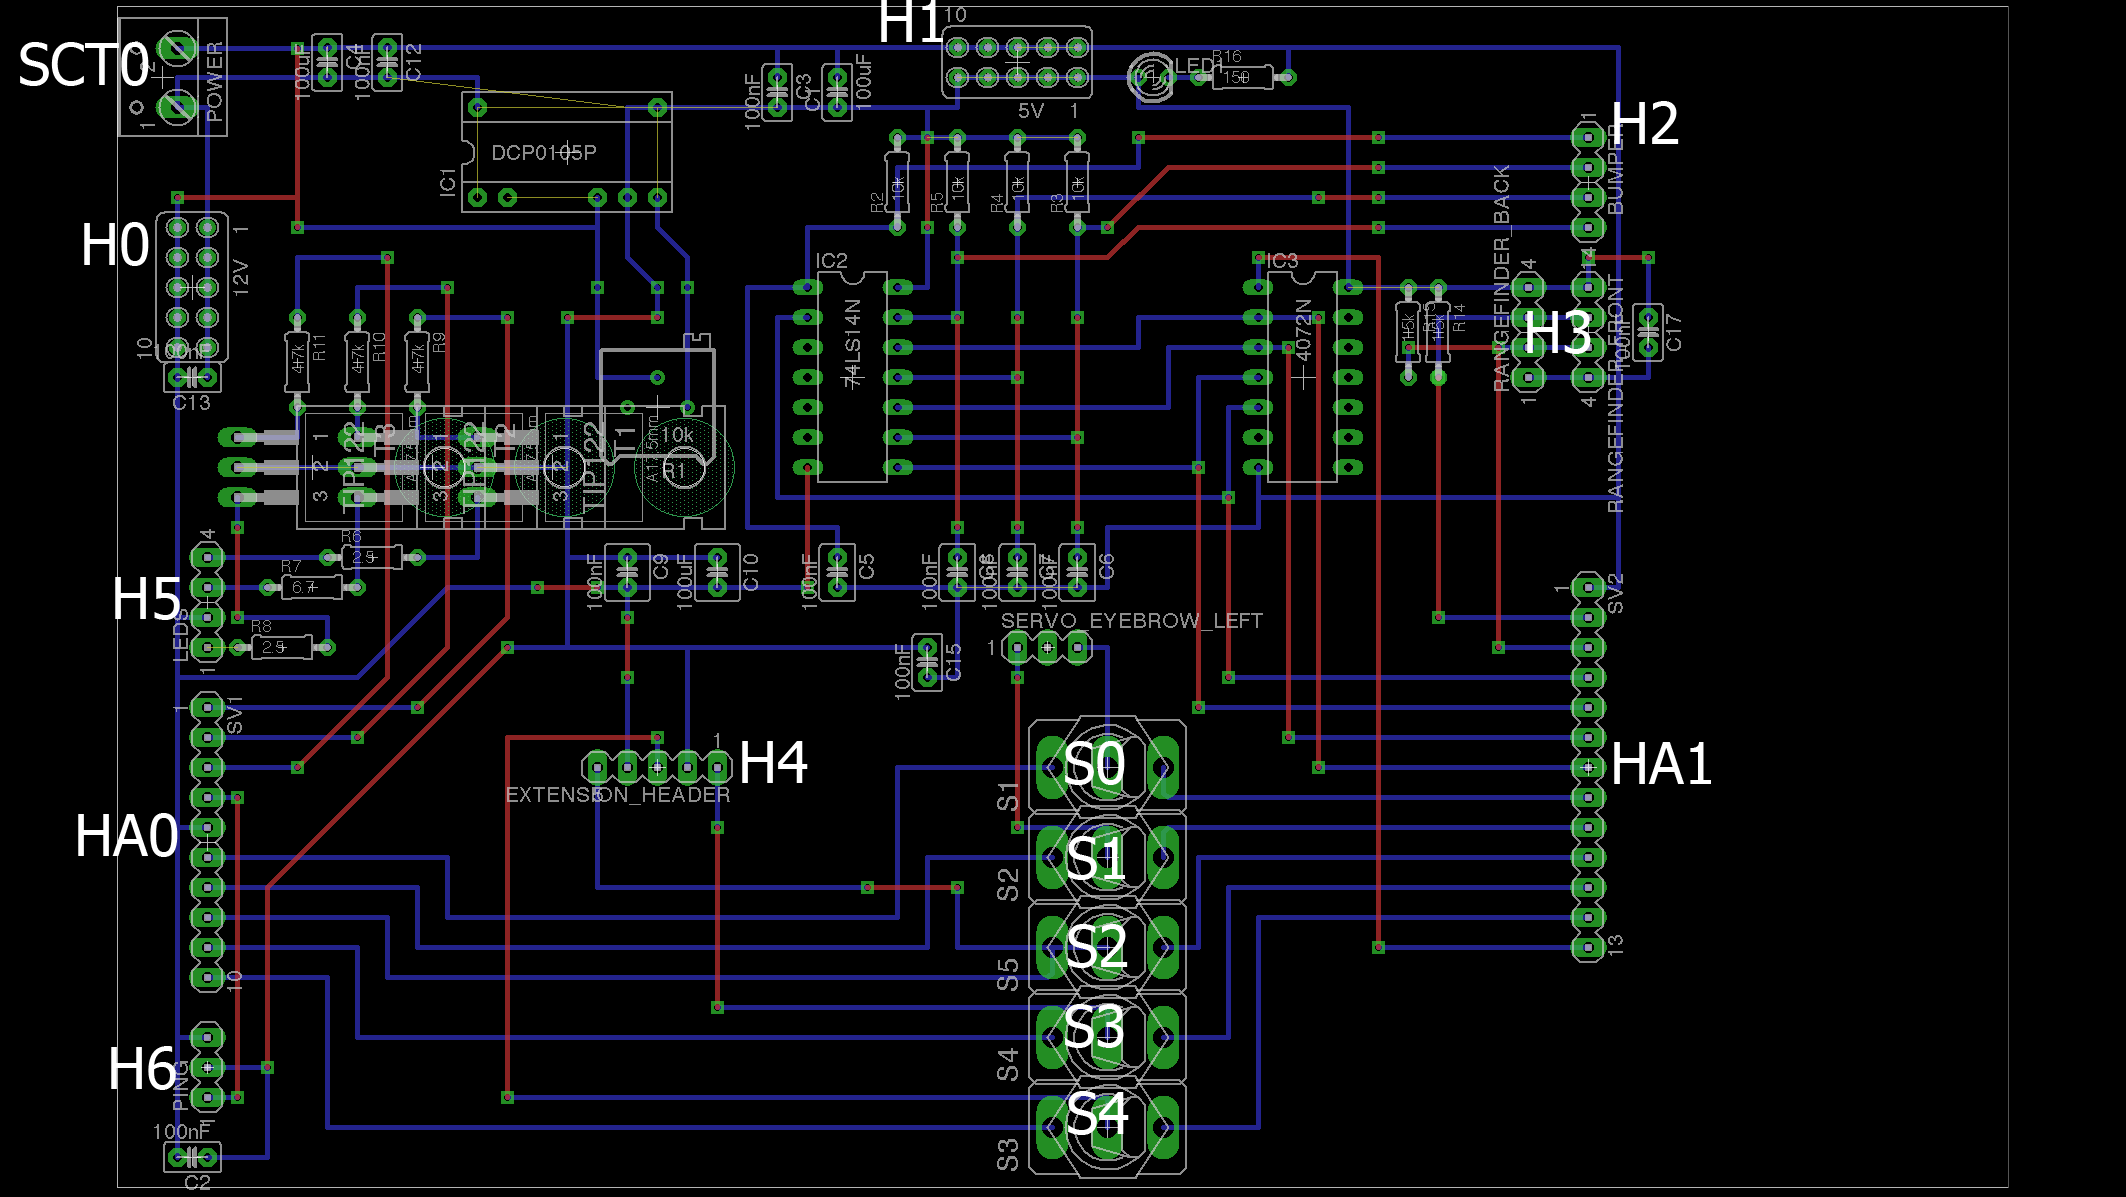
\includegraphics[scale=1.1]{Images/MainBoard_Specs.png}}
	\caption{Main board layout}
	\label{fig:main_board_layout}
\end{figure}

\begin{table}[ht!]
\begin{minipage}[b]{0.5\linewidth}
  \begin{tabular}{| l | c | r |}
    \hline
    {\bf Header} 		& 		{\bf Pin} 		& 	{\bf Function} 		\\ \hline
    {\bf SCT0} 		& 	 				&  	Main power 		\\ \hline
     				&		1 			&	12V				\\ \hline
     				&		2 			& 	Ground 			\\ \hline
   {\bf H0} 			&	 				& 	12V Distribution 	\\ \hline
     	 			& 		odd 			&	12V 				\\ \hline
    	 			&		even	 		&	Ground 			\\ \hline
   {\bf H1}	 		&	 				&	5V Distribution 		\\ \hline
    				& 		odd 			&	5V				\\ \hline
    	 			&		even 		&	Ground 			\\ \hline
   {\bf H2}	 		&	 				&	Bumper buttons 	\\ \hline 
   				&		1			&       Front button		\\ \hline
				&		2			&	Rear	 button		\\ \hline
				&		3			&	Left button		\\ \hline
				&		4			&	Right button		\\ \hline
  {\bf H3}	 		&	 				&	SRF02 I2C bus 	\\ \hline 
   				&		1			&       Ground			\\ \hline
				&		2			&	SCL				\\ \hline
				&		3			&	SDA				\\ \hline
				&		4			&	5V				\\ \hline
 {\bf H4}	 		&	 				&	Spare Header		\\ \hline 
   				&		1			&       Arduino pin		\\ \hline
				&		2			&	5V				\\ \hline
				&		3			&	Arduino pin		\\ \hline
				&		4			&	Ground			\\ \hline
				&		5			&	Arduino Pin		\\ \hline
{\bf H5}	 		&	 				&	RGB LED Header	\\ \hline 
   				&		1			&       Blue				\\ \hline
				&		2			&	Ground			\\ \hline
				&		3			&	Red 				\\ \hline
				&		4			&	Green			\\ \hline
 \end{tabular}	
 \end{minipage}
   \hspace{2mm}
   \begin{minipage}[b]{0.5\linewidth}
   \begin{tabular}{| l | c | r |}
   \hline
    {\bf Header} 		& 		{\bf Pin} 		& 	{\bf Function} 		\\ \hline	
 {\bf H6}	 		&	 				&	Ping Header		\\ \hline 
   				&		1			&       Ping signal		\\ \hline
				&		2			&	5V				\\ \hline
				&		3			&	Ground			\\ \hline
 {\bf HA0}	 		&	 				&	Arduino Header 0	\\ \hline 
   				&		1			&      	Green PWM 		\\ \hline
				&		2			&	Red PWM			\\ \hline
				&		3			&	Blue PWM		\\ \hline
				&		4			&	Ping	signal		\\ \hline
				&		5			&	Ground			\\ \hline
				&		6			&	Left eyebrow servo	\\ \hline
				&		7			&	Right eyebrow servo	\\ \hline
				&		8			&	Extra pin			\\ \hline
				&		9			&	Extra pin			\\ \hline
				&		10			&	Extra pin			\\ \hline
 {\bf HA1}	 		&	 				&	Arduino Header 1	\\ \hline 
   				&		1			&       Ground			\\ \hline
				&		2			&	SDA				\\ \hline
				&		3			&	SCL				\\ \hline
				&		4			&	Bumper front		\\ \hline
				&		5			&	Bumper rear		\\ \hline
				&		6			&	Bumper left		\\ \hline
				&		7			&	Bumper right		\\ \hline
				&		8			&	Left eyebrow servo	\\ \hline
				&		9			&	Right eyebrow servo	\\ \hline
				&		10			&	Extra pin			\\ \hline
				&		11			&	Extra pin			\\ \hline
				&		12			&	Extra pin			\\ \hline
				&		13			&	Bumper interrupt trigger	\\ \hline
				
				
  \end{tabular}
  \end{minipage}
\caption{Main Board Connectors}
\label{tab:mainBoardConnectors}
\end{table}


\subsection{5V}
The  LSM2-T/10-D12N-C  DC/DC converter serves as the $5V$ power supply. This device can be configured to $5V$ with a resistor connected between the ground pin and the trim pin. A resistance of $1.472 k\Omega$ is needed for a $5V$ output. So a $3k\Omega$ potentiometer is put in place to accommodate the desired resistance.


 \newpage
\subsection{RGB Control}
The light in Eva's head is generated by twelve $10mm$ RGB LEDs on each side. The actual color of the LEDs is controlled by a pwm signal from the Arduino. TIP121 Darlington transistors amplify this signal to provide enough current to the 24 LEDs.

Each LED actually consists of three LEDs. A red one, a green one and a blue one. They all consume a maximum of $20 mA$. That sums up to $480mA$ for all the LEDs combined. The red LEDs drop $1.8V$ and the green and blue LEDs drop $3.8V$. So to limit the current two different resistor values are needed.

\begin{equation*}
Rred =  \frac{Vcc-Vred}{Ired*24} = \frac{5-1.8}{0.020*24} = 6.7 \Omega
\end{equation*}
\begin{equation*}
Rgreen = \frac{Vcc-Vgreen}{Igreen*24} =\frac{5-3.8}{0.020*24} = 2.5 \Omega
\end{equation*}
\begin{equation*}
Rblue = \frac{Vcc-Vblue}{Iblue*24} =\frac{5-3.8}{0.020*24} = 2.5 \Omega
\end{equation*}

Note that it is a rather na�ve implementation to link all LEDs to only one resistor. Since the current through the other LEDs will increase if one of them breaks down causing others to break down as well. The proper way to implement this would be to insert a resistor before every LED.

The Darlington transistors only need a small amount of current at their base. 4.7$k\Omega$ resistors are chosen to limit the base current to $1 mA$. The Darlingtons have a $h_{fe}$ of 1000 so the maximum current they can provide is 1 * 1000 = 1000 $mA$ which is enough.

 
 
 
\subsection{Data Acquisition}
Eva�s bumper detects bumps by six buttons around the mobile base that provide 4 signals: front, rear, left and right. These signals are guided through a debouncing circuit(Figure \ref{fig:DAQ}). The capacitors keep the voltage to $5V$ when the buttons are not pressed. The Schmitt Trigger converts the signal to a logical zero.
When a button is pressed it will connect the anode side of the capacitor to the ground. This will cause the charge in the capacitor to flow away and pull the signal low. Then the Schmitt Trigger will swing its signal high.  

These stable signals are fed to a 4-input OR port. The output of this OR port triggers an interrupt on the Arduino, which subsequently reads the button signals to determine which bumper has been hit. 
 
 \begin{figure}[ht!]
	\centering
	\mbox{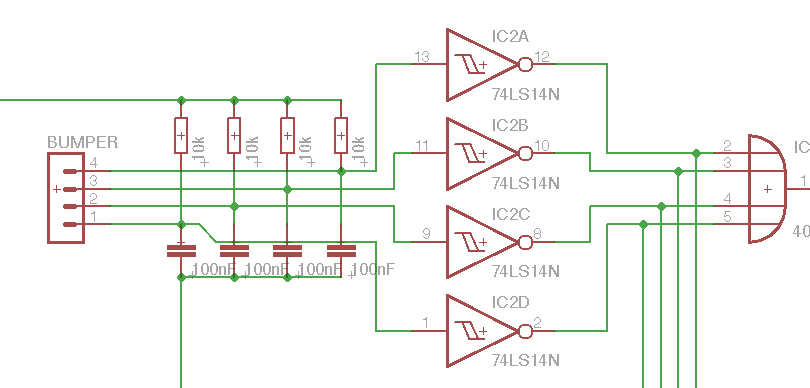
\includegraphics[scale=0.5]{Images/DAQ.png}}
	\caption{Debouncing Circuit}
	\label{fig:DAQ}
\end{figure}

Other data acquisition done on the main board is the reading of the ultrasonic Ping sensor attached to the gripper and the 10 SRF02 sensors, which are also ultrasonic range finders.
The Ping has to be triggered with a 5$\mu$s pulse and returns a high pulse with a duration that matches the time of flight on the same pin.
The SRF02 sensors are all connected on an I2C bus. They are fired in two phases. First al even ones do a distance measurement then all odd sensors do theirs. This is to prevent interference of neighboring sensors.

\subsection{Servos}
The main board�s final function is to power the servos in Eva�s head and to perform as a hatch for Arduino signals controlling the servos. Also there are three vacant pins to attach more devices if desired.

 \begin{figure}[ht!]
	\centering
	\mbox{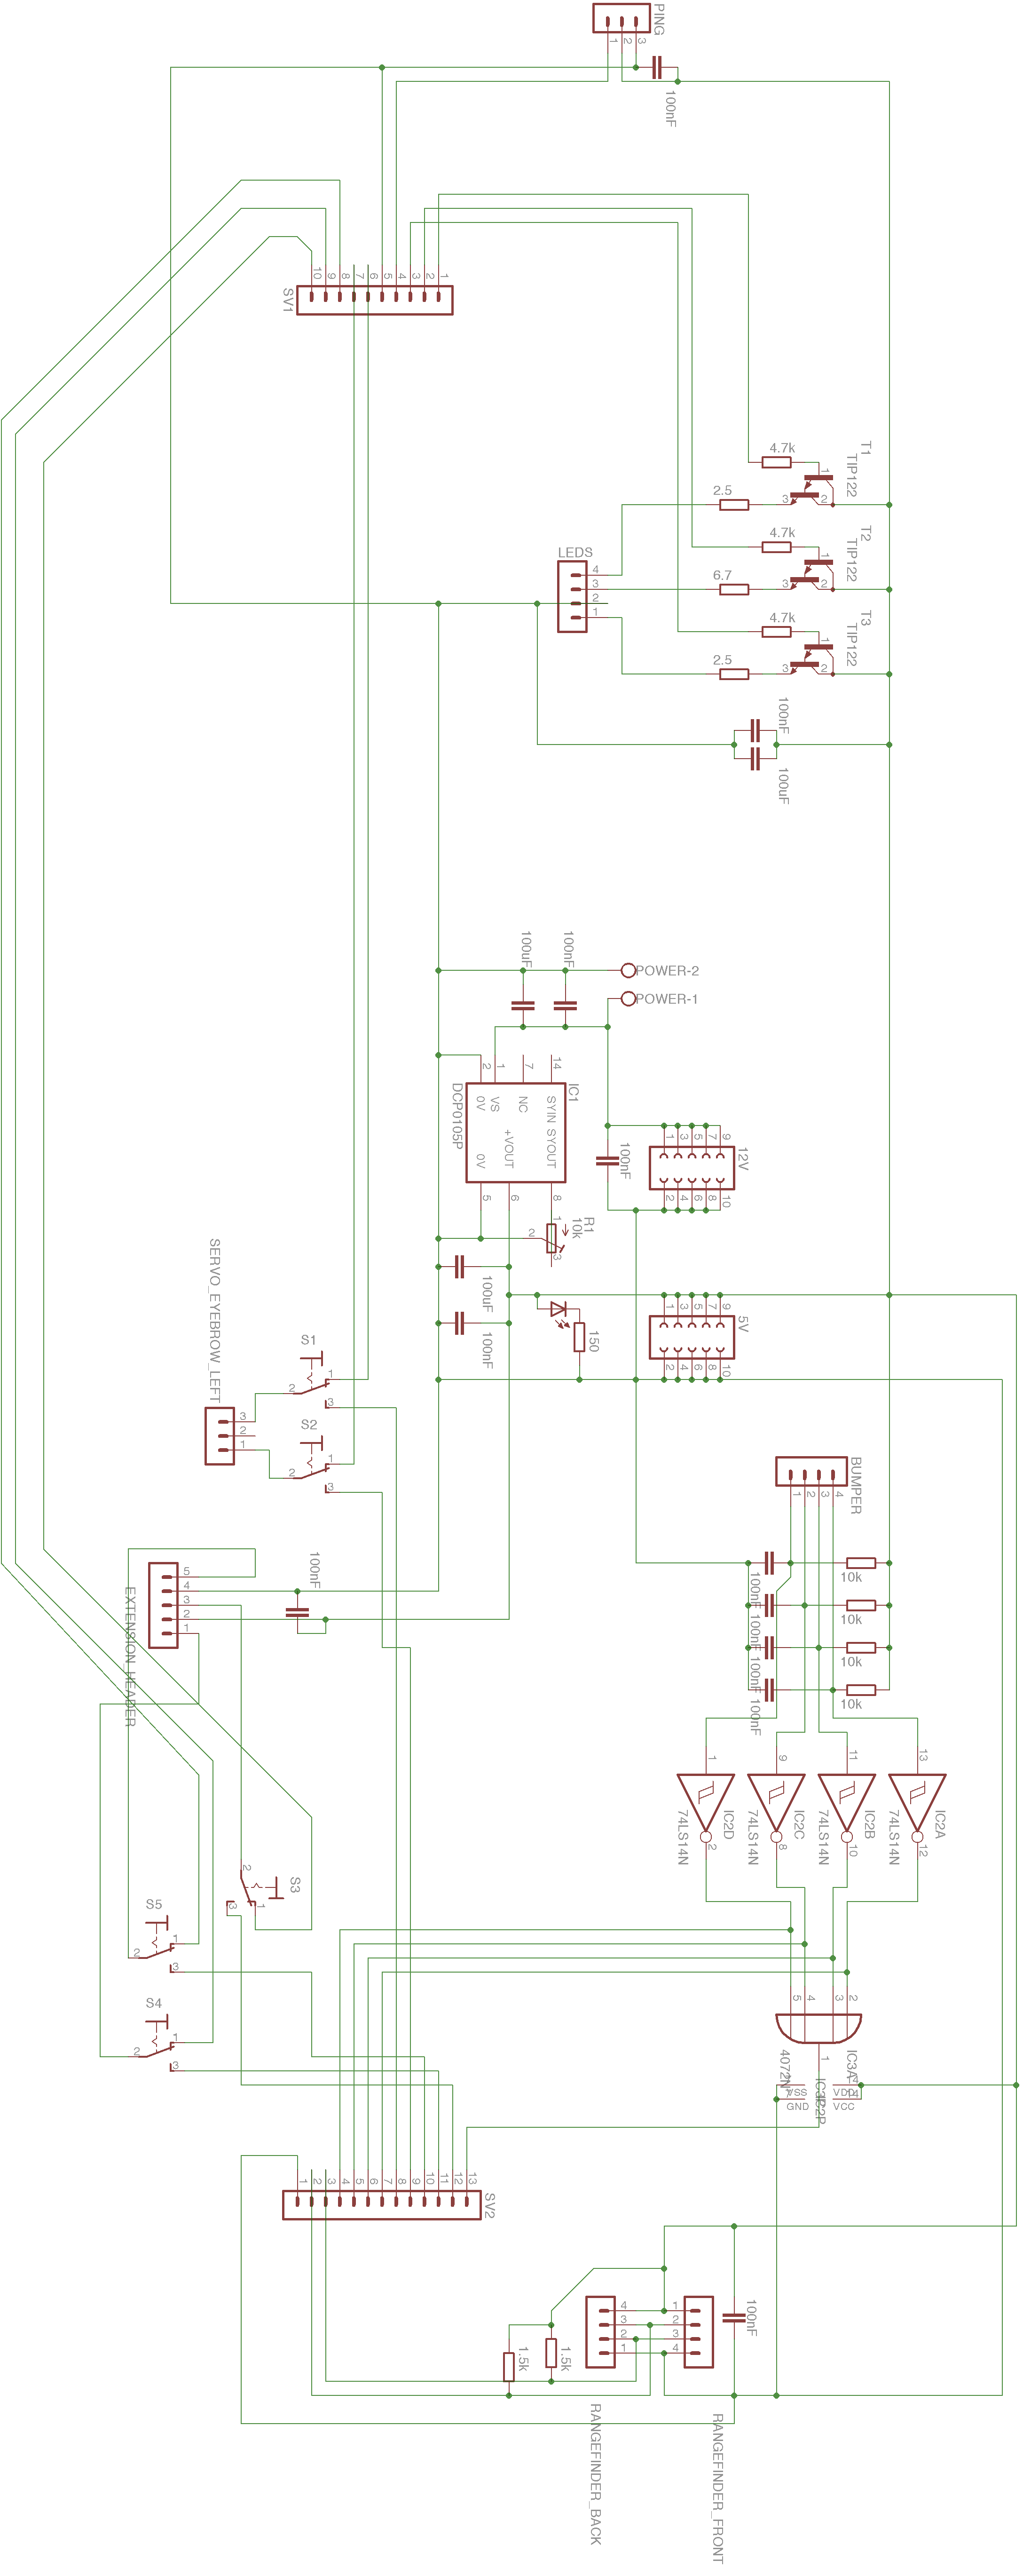
\includegraphics[scale=0.47]{Images/MainBoardSchematic.png}}
	\caption{Main Board Schematic}
	\label{fig:MBS}
\end{figure}


\end{document}